\chapter{摘要}
GAN(Generative Adversarial Network)自提出之时候就备受的深度学习的关注。和判别模
型不同, GAN不需要数据具有标签,它试图解
决的问题是如何根据现有的数据生成的数据集中间从来都没有数据, 但是该数据和数据集
中间的数据类似。在本课设中间, 将会使用MNIST和各种自制的几何图形来验证和分析
GAN的能力。

\section{选题背景}
GAN是Ian Goodfellow在2004年提出的神经网络模型,该模型可以通过Discriminator 和
Generator的两个神经网络的对抗学习,通过现用的数据生成出新的数据。 Discriminator
网络是一个用于判别的网络,输入为数据X, 输出为一个bool值, 当该bool值表示该数据是
的Generator创造的伪造的数据否者是从数据库中随机取出来的数据。Generator的输入为随
机噪音, 输出值为伪造的数据。\\
    GAN无论是从理论上还是从应用上都具有高意义。 GAN利用了博弈论的思想,
Discriminator 和 Generator两者互相博弈, 让Discriminator的判别能力逐步强化, 而
同时让Generator生成图片逐步和测试的样例中间的图片的更加相似。GAN启发研究者, 只
有通过坚实的理论基础, 采用可能打开的深度学习的新大门。 当GAN可以通过的噪音获取
到正确的图形的时候, 说明Generator已经可以抓取到数据库中间的数据分布的特点,而先
用的分类器的分类的依据也是通过不同标签的数据分布的位置不同, 从而实现对于数据的
分类的。 GAN的应用非常的广泛, 包括的字体生成,文字到图片的装换,实时人脸重建等
等应用。\\
    在本次课设中, 使用MNIST以及多种自己创建的数据, 用于测试GAN在具体的样本上的能力
如何, 通过多种简单几何图形的数据集的测试,比对GAN对于特殊的几何的图形的性质是否
同样可以识别并且生成出来
。


\section{理论介绍}
理解GAN, 首先需要理解生成模型和判别模型直接的区别是什么:
公式$p(y|x)$ 用于描述“给定x, y的概率是多少”,在MNIST中间,其含义是给定一张图片,
该数字是0的可能性。而$p(x|y)$的用于表示给定出一个类, 该类数据的含有特定特征的概
率。\\
G(Generator)和Discriminator(D)的分别是两个神经网络, 前者使用生成模型,后者
使用判别模型。如图\ref{algorithm}所示,G使用latent space和噪音混合输入, 然
后生成出来伪造数据, 混合在真实数据中让D来分辨。
\begin{figure}[!hbt]
    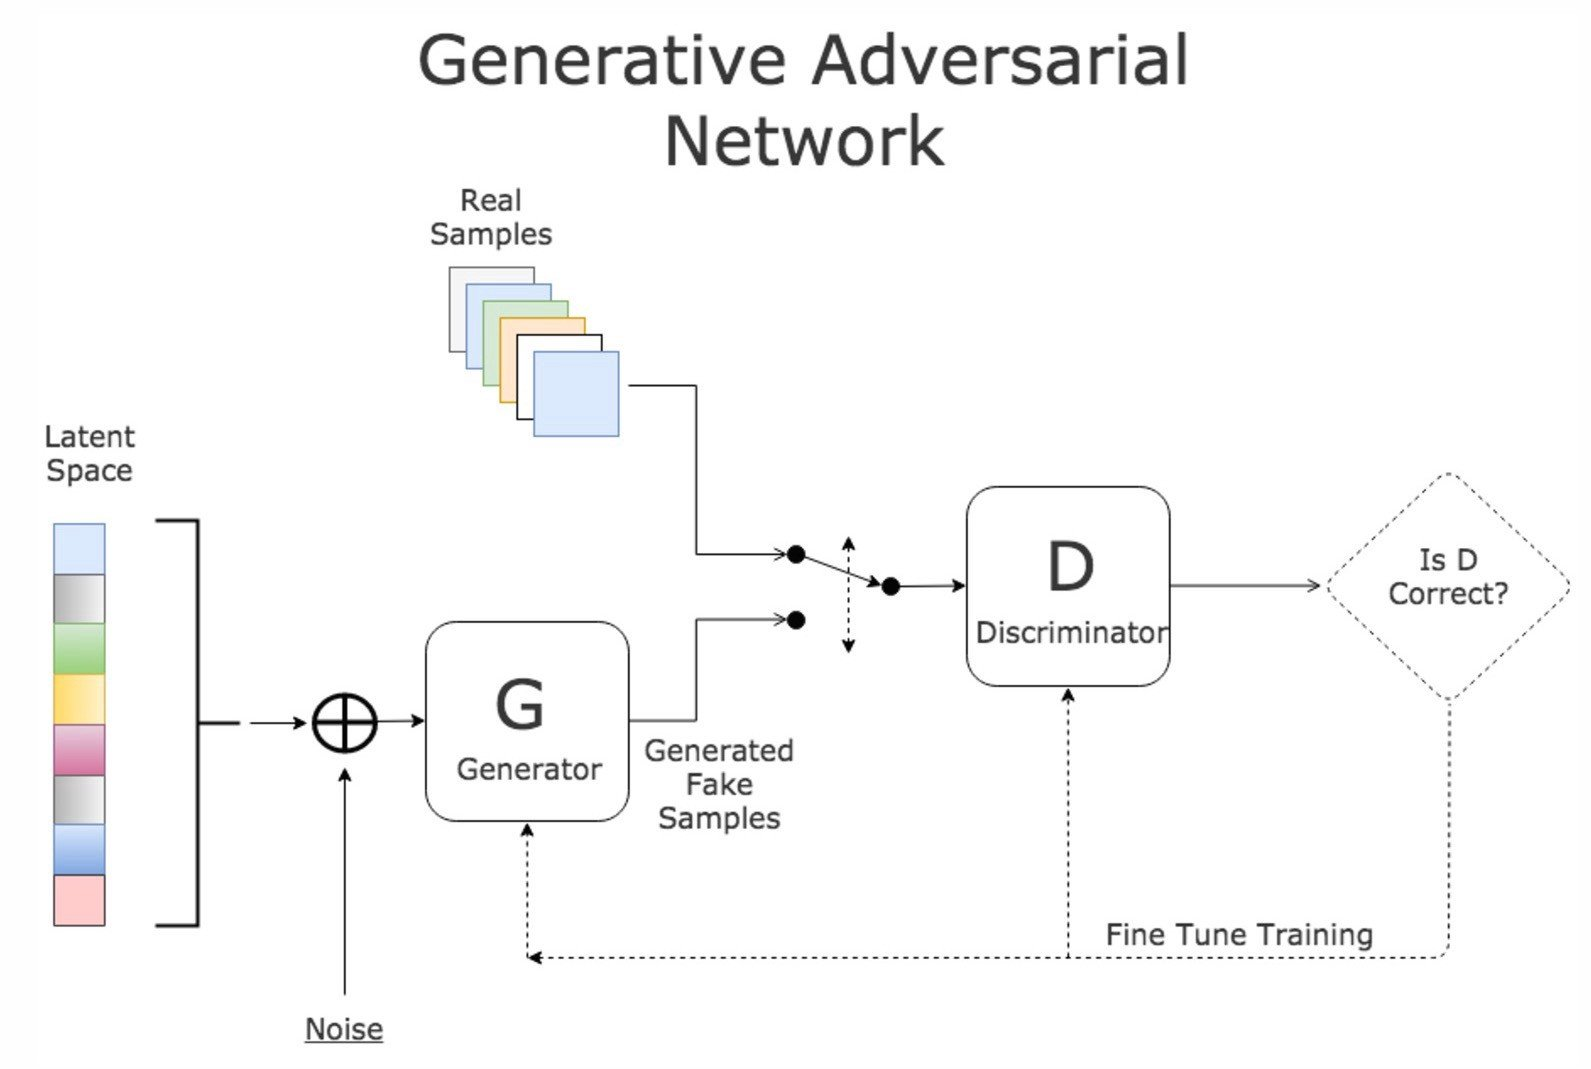
\includegraphics[width=\linewidth]{pic/algo.jpg}
    \caption{GAN}
    \label{algorithm}
\end{figure}
但使用MNIST的数据集合的时候,该具体化为\ref{m_algorithm}所示的结果。
\begin{figure}[!hbt]
    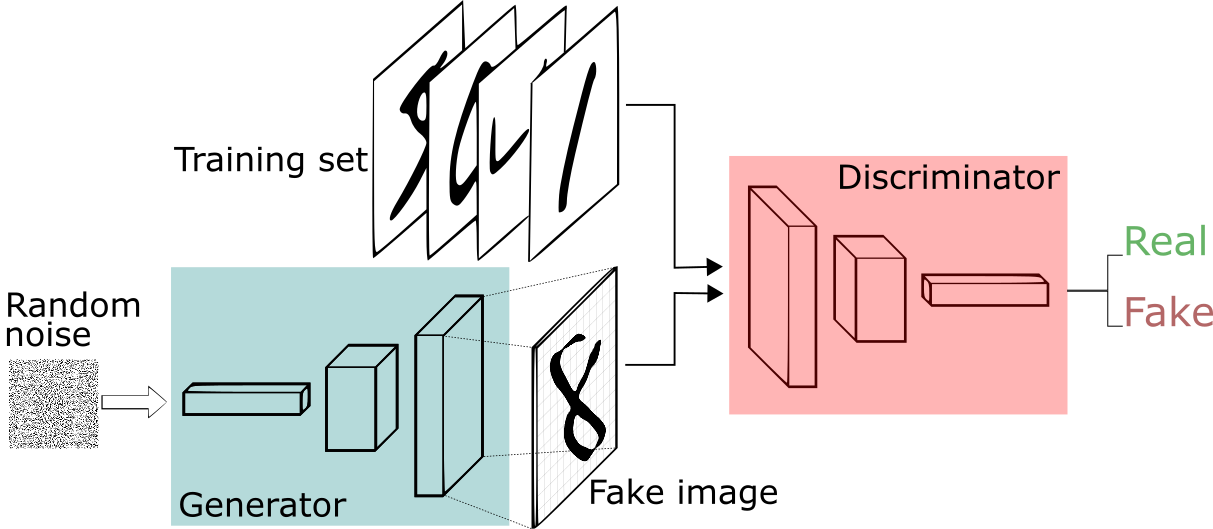
\includegraphics[width=\linewidth]{pic/mnist_algo.png}
    \caption{GAN with mnist}
    \label{m_algorithm}
\end{figure}
\newline
该算法的具体描述\ref{algo-1}, 从该算法需要注意的是, 总是多次训练D然后在训练一次
G, 其中原因是为了让D更快获取较强的分类能力, 避免陷入到分类器D和生成器G的能力都
的不高的状态中间。
\begin{figure}[!hbt]
    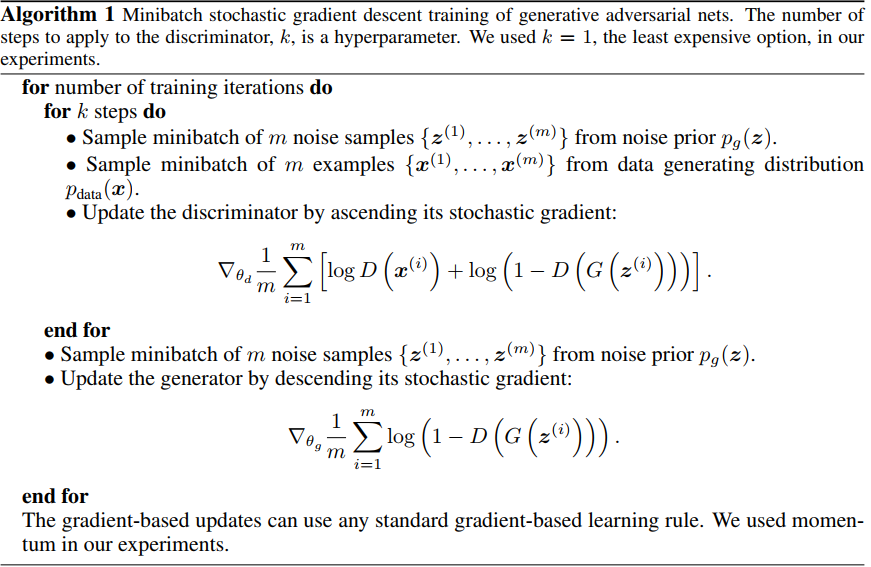
\includegraphics[width=\linewidth]{pic/algo-1.png}
    \caption{GAN algorithm}
    \label{algo-1}
\end{figure}
\newline
此算法的来源是\ref{formualtion}中公式, 对于目标公式,G 和 D 分别将该的公式最大
化和最小化,希望达到的结果G可以产生近似真实的图片,而D可以具有很强分类能力。
\begin{figure}[!hbt]
    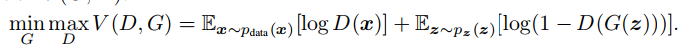
\includegraphics[width=\linewidth]{pic/for.png}
    \caption{GAN formula}
    \label{formualtion}
\end{figure}
\newline


\section{参考文档}
\begin{itemize}
    \item https://deeplearning4j.org/generative-adversarial-network
    \item https://arxiv.org/pdf/1701.00160.pdf
    \item https://github.com/nashory/gans-awesome-applications
    \item https://arxiv.org/pdf/1703.10580v1.pdf
    \item http://yann.lecun.com/exdb/mnist/
\end{itemize}
